\chapter{ЕКСПЕРИМЕНТАЛЬНІ ДОСЛІДЖЕННЯ}
Ми оцінюємо можливості репрезентативного навчання
ResNet, Vision Transformer (ViT) та гібриду.
Щоб зрозуміти вимоги до даних кожної моделі, ми попередньо
тренуємось на наборах даних різного розміру та оцінюємо багато
контрольних завдань. Розглядаючи обчислювальні витрати на
попереднє тренування моделі, ViT працює дуже вигідно,
досягаючи кращих методів за більшістю тестів розпізнавання
за нижчої вартості попереднього тренування. Нарешті, ми проводимо
невеликий експеримент, використовуючи самоконтроль,
і показуємо, що самоувага ViT є перспективною.

\section{Налаштування}
\subsection{Датасети}
Для дослідження масштабованості моделі ми використовуємо
набір даних ILSVRC-2012 ImageNet з 1 тис. класами та 1,3 млн. зображеннями
(далі ми називаємо його ImageNet), його надмножину ImageNet-21k
з 21 тис. класами та 14 млн. зображеннями та JFT з 18 тис. 
класів та 303 млн. зображень із високою роздільною здатністю.
Ми видаляємо дублікати даних попередньої підготовки
відносно тестових наборів даних поточних завдань.
Ми переносимо моделі, навчені цим набором даних, на кілька базових завдань:
ImageNet на оригінальних мітках перевірки та очищених мітках ReaL,
CIFAR-10/100, Oxford-IIIT Pets та Oxford Flowers-102.

\subsection{Варіанти моделі}
Ми базуємо конфігурації ViT на тих, що використовуються для
BERT \cite{bert}, як описано в таблиці \ref{tab:t1}.
Моделі ``Base'' та ``Large'' безпосередньо беруться від BERT,
і ми додаємо більшу модель ``Huge''. Далі ми використовуємо
короткі позначення для позначення розміру моделі
та розміру вхідного регіону: наприклад, ViT-L/16 означає ``Large''
варіант із розміром вхідного патча $16 \times 16$.
Зауважте, що довжина послідовності трансформера
обернено пропорційна квадрату розміру регіона,
тому моделі з меншим розміром патча обчислювально дорожчі.

Для базових CNN ми використовуємо ResNet,
але замінюємо шари пакетної нормалізації
на групову нормалізацію і використовуємо стандартизовані згортки.
Для гібридів ми подаємо проміжні репрезентації у ViT з
розміром регіона один ``піксель''.

\begin{table}[H]
    \caption{Деталі варіантів моделі}
    \begin{tabular}{ c c c c c c }
        \hline
        Модель & Шари & Прихов. розмір $D$ & Розм. щільн. шару & Голов. & Парам.  \\ \hline
        ViT-Base & 12 & 768 & 3072 & 12 & 86M  \\ 
        ViT-Large & 24 & 1024 & 4096 & 16 & 307M  \\ 
        ViT-Huge & 32 & 1280 & 5120 & 16 & 632M  \\ \hline
    \end{tabular}
    \label{tab:t1}
\end{table}

\subsection{Навчання та точне налагодження}
Ми тренуємо всі моделі, включаючи ResNet, за допомогою Adam
з $\beta_1 = 0.9$, $\beta_2 = 0.999$, пеакетний розмір 4096 та вагою розпаду
$0.1$. Для точкого налагодженн ми використовуємо SGD з імпульсом,
розмір пакету 512, для всіх моделей.

\section{Порівняння з кращими сучасними методами}
Спочатку ми порівнюємо наші найбільші моделі 
-- ViT-H/14 та ViT-L/16 --
із найсучаснішими CNN з літератури. Першим пунктом порівняння є
Big Transfer (BiT) \cite{big-transfer}, який виконує навчання
з вчителем для переходу з великими ResNets.
Другий - Noisy Student, який є великим EfficientNet, який навчається
за допомогою напівконтрольного навчання на ImageNet та JFT-300M зі
знятими мітками. В даний час Noisy Student є найсучаснішим на
ImageNet та BiT-L для інших наборів даних, про які повідомляється тут.
Усі моделі пройшли навчання на апаратному забезпеченні TPUv3,
і ми повідомляємо про кількість днів, ядер TPUv3, необхідних
для попереднього тренування кожного з них, тобто про
кількість ядер TPU v3 (2 на чіп), помножених на час навчання в днях.

У таблиці \ref{tab:t2} наведені результати.
Менша модель ViT-L/16, попередньо навчена на JFT-300M,
перевершує BiT-L (яка попередньо навчена на тому самому наборі даних)
у всіх завданнях, вимагаючи при цьому значно менших обчислювальних
ресурсів для навчання. Більша модель, ViT-H/14, додатково покращує
продуктивність, особливо на більш складних наборах даних
-- ImageNet, CIFAR-100 та наборі VTAB. Цікаво, що модель все ще
вимагала значно менших обчислень для попереднього тренування,
ніж попередні сучасні моделі. Нарешті, модель ViT-L/16, попередньо
навчена на загальнодоступному наборі даних ImageNet-21k, також
добре працює на більшості наборів даних, при цьому вимагає 
менше ресурсів для попередньго тренування.

\begin{table}[H]
    \caption{Порівняння з кращими сучасними методами (1)}
    \begin{tabular}{ c c c }
        \hline
         & Ours-JFT (ViT-H/14) & Ours-JFT (ViT-L/16)  \\ \hline
        ImageNet           & 88.55 & 87.76  \\ 
        ImageNet ReaL      & 90.72 & 90.54   \\ 
        CIFAR-10           & 99.50 & 99.42  \\ 
        Oxford-IIIT Pets   & 94.55 & 93.90  \\ 
        Oxford Flowers-102 & 97.56 & 97.32  \\ 
        VTAB (19 задач)    & 99.68 & 99.74  \\ \hline
        TPUv3-core-days    & 77.63 & 76.28  \\ \hline
    \end{tabular}
    \label{tab:t2}
\end{table}

\begin{table}[H]
    \caption{Порівняння з кращими сучасними методами (2)}
    \begin{tabular}{ c c }
        \hline
         & Ours-121k (ViT-L/16)  \\ \hline
        ImageNet           & 85.30   \\ 
        ImageNet ReaL      & 88.62   \\ 
        CIFAR-10           & 99.15   \\ 
        Oxford-IIIT Pets   & 93.25   \\ 
        Oxford Flowers-102 & 94.67   \\ 
        VTAB (19 задач)    & 99.61   \\ \hline
        TPUv3-core-days    & 72.72   \\ \hline
    \end{tabular}
    \label{tab:t3}
\end{table}

\begin{table}[H]
    \caption{Порівняння з кращими сучасними методами (3)}
    \begin{tabular}{ c c c }
        \hline
         & BiT-L (ResNet152x4) & Noisy Student (EfficientNet-L2)  \\ \hline
        ImageNet           & 87.54 & 88.4  \\ 
        ImageNet ReaL      & 90.54 & 90.55  \\ 
        CIFAR-10           & 99.37 & --  \\ 
        Oxford-IIIT Pets   & 93.51 & --  \\ 
        Oxford Flowers-102 & 96.62 & --  \\ 
        VTAB (19 задач)    & 99.63 & --  \\ \hline
        TPUv3-core-days    & 78.29 & --  \\ \hline
    \end{tabular}
    \label{tab:t4}
\end{table}

\section{Огляд Vision Transformer}
Щоб почати розуміти, як Vision Transformer обробляє дані
зображення, ми аналізуємо його внутрішні уявлення. Перший шар
Vision Transformer лінійно проектує розгорнуті плями в простір
нижчих розмірів (рівняння \ref{eq:1}).
На рисунку \ref{fig:filters} (зліва) показано основні
компоненти вивчених фільтрів ембедингу.
Компоненти нагадують правдоподібні базові функції
для низьковимірного представлення тонкої структури в кожному
регіоні.

\begin{figure}[H]
    \centering
    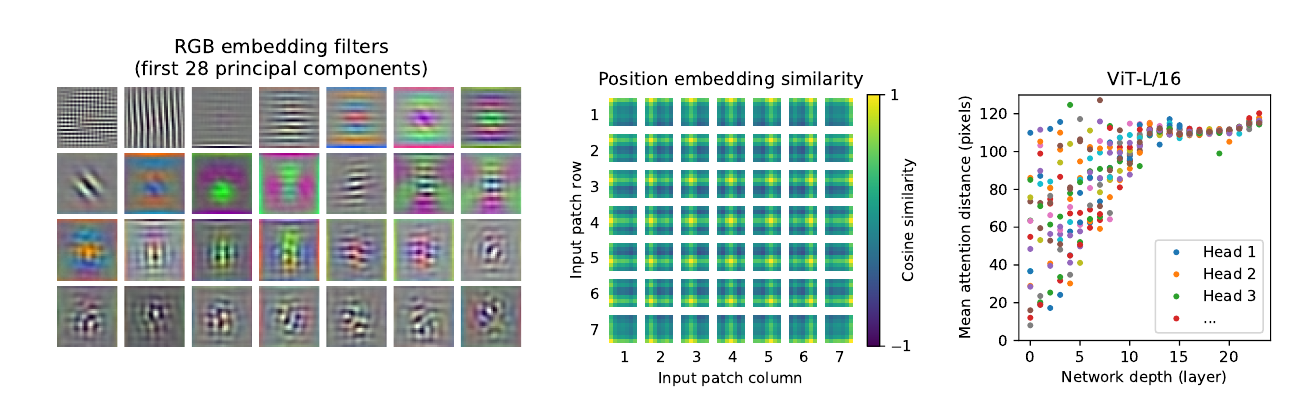
\includegraphics[width=1\textwidth]{filters.png}
    \caption{Фільтри початкового лінійного ембедингу, схожість позиційних ембедингів, розмір площі, якій головка приділяє увагу}
    \label{fig:filters}
\end{figure}

Після проекції до представлення регіонів зображення додається
позиціонний ембедінг. Рисунок \ref{fig:filters} (в центрі) показує,
що модель вчиться кодувати відстань всередині зображення за схожістю
позиційних ембедингів, тобто ближчі регіони, як правило, мають більше
подібних позиційних ембедингів. Далі з'являється структура рядка-стовпця;
регіони в одному рядку/стовпці мають подібні ембедінги.
Нарешті, синусоїдальна структура іноді виявляється для більших сіток.
Те, що позиційні ембедінги вчаться представляти
топологію 2D-зображень, пояснює, чому власноруч
створені 2D варіанти ембедингів не дають
вдосконалення.

Самоувага дозволяє ViT інтегрувати інформацію по всьому
зображенню навіть у найнижчих шарах. Ми досліджуємо, наскільки мережа
використовує цю можливість. Зокрема, ми обчислюємо середню
відстань у просторі зображення, через яку інтегрується інформація,
на основі ваг уваги (рисунок \ref{fig:filters}, праворуч).
Ця ``відстань уваги'' є аналогом розміру сприйнятливого поля в ЗНМ.
Ми виявили, що деякі головки придають увагу більшій частині зображення
вже на найнижчих шарах, показуючи, що модель справді
використовує здатність інтегрувати інформацію глобально.
Інші головки уваги мають постійно малі відстані уваги в низьких шарах.
Ця сильно локалізована увага менш виражена у гібридних моделях,
які застосовують ResNet перед трансформером
(Рисунок \ref{fig:filters}, праворуч), що припускає, що він може
виконувати подібну функцію, як ранні згорткові шари в ЗНМ.
Далі, відстань уваги зростає із збільшенням глибини мережі.
Глобально ми виявили, що модель враховує області зображень,
які є семантично важливими для класифікації
(рисунок \ref{fig:attention-repr}).

\begin{figure}[H]
    \centering
    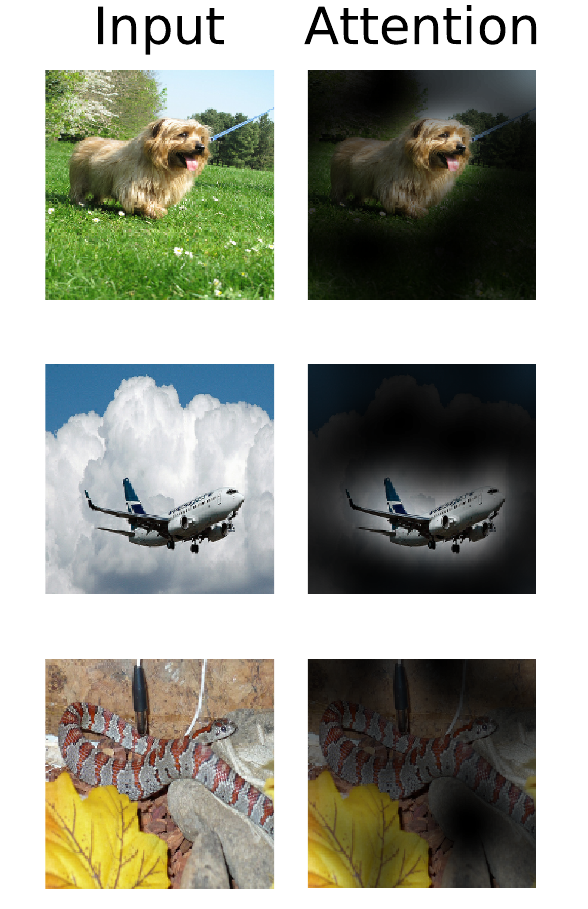
\includegraphics[width=0.3\textwidth]{attention-repr.png}
    \caption{Приклади уваги з вихідного токену то вхідного простору}
    \label{fig:attention-repr}
\end{figure}
